\documentclass[letterpaper,11pt,oneside,reqno]{article}

%%%%%%%%%%%%%%%%%%%%%%%%%%%%%%%%%%%%%%%%%%%%%%%%%%%%%%%%%%%%

\usepackage[pdftex,backref=page,colorlinks=true,linkcolor=blue,citecolor=red]{hyperref}
\usepackage[alphabetic,nobysame]{amsrefs}

%%%%%%%%%%%%%%%%%%%%%%%%%%%%%%%%%%%%%%%%%%%%%%%%%%%%%%%%%%%%
%main packages
\usepackage{amsmath,amssymb,amsthm,amsfonts,mathtools}
\usepackage{graphicx,color}
\usepackage{upgreek}
\usepackage[mathscr]{euscript}

%equations
\allowdisplaybreaks
\numberwithin{equation}{section}

%tikz
\usepackage{tikz}
\usetikzlibrary{shapes,arrows,positioning,decorations.markings}
\usepackage{pgfplots}
\pgfplotsset{compat=1.18}

%conveniences
\usepackage{array}
\usepackage{adjustbox}
\usepackage{cleveref}
\usepackage{enumerate}
\usepackage{datetime}

%paper geometry
\usepackage[DIV=12]{typearea}

%%%%%%%%%%%%%%%%%%%%%%%%%%%%%%%%%%%%%%%%%%%%%%%%%%%%%%%%%%%%
%draft-specific
\synctex=1
% \usepackage{refcheck,comment}

%%%%%%%%%%%%%%%%%%%%%%%%%%%%%%%%%%%%%%%%%%%%%%%%%%%%%%%%%%%%
%this paper specific
\newcommand{\ssp}{\hspace{1pt}}

%%%%%%%%%%%%%%%%%%%%%%%%%%%%%%%%%%%%%%%%%%%%%%%%%%%%%%%%%%%%
\newtheorem{proposition}{Proposition}[section]
\newtheorem{lemma}[proposition]{Lemma}
\newtheorem{corollary}[proposition]{Corollary}
\newtheorem{theorem}[proposition]{Theorem}
%%%%%%%%%%%%%%%%%%%%%%%%%%%%%%%%%%%%%%%%%%%%%%%%%%%%%%%%%%%%
\theoremstyle{definition}
\newtheorem{definition}[proposition]{Definition}
\newtheorem{remark}[proposition]{Remark}
%%%%%%%%%%%%%%%%%%%%%%%%%%%%%%%%%%%%%%%%%%%%%%%%%%%%%%%%%%%%

\begin{document}
\title{Lectures on Random Matrices
(Spring 2025)
\\Lecture 11: Some universal asymptotics of Dyson Brownian Motion}


\date{March 26, 2025\footnote{\href{https://lpetrov.cc/rmt25/}{\texttt{Course webpage}}
$\bullet$ \href{https://lpetrov.cc/simulations/model/random-matrices/}{\texttt{Live simulations}}
$\bullet$ \href{https://lpetrov.cc/rmt25/rmt25-notes/rmt2025-l11.tex}{\texttt{TeX Source}}
$\bullet$
Updated at \currenttime, \today}}



\author{Leonid Petrov}


\maketitle
\tableofcontents

\section{Recap}

\subsection{Dyson Brownian Motion (DBM)}
We introduced a time-dependent model of random matrices by letting an
\(N\times N\) Hermitian matrix \(\mathcal{M}(t)\) evolve in time so that each
off-diagonal entry follows independent Brownian increments (real or complex
depending on the symmetry class).  Setting
\[
\mathcal{M}(t) \;=\; \frac{1}{\sqrt{2}}\bigl(X(t) + X^\dagger(t)\bigr),
\]
where \(X(t)\) is an \(N\times N\) matrix of i.i.d.\ Brownian motions,
produces a self-adjoint matrix with a stochastically evolving spectrum.
This model is full-rank matrix Brownian motion,
and works well for $\beta=1,2,4$.
For other $\beta$, we need an SDE to describe the evolution of the eigenvalues (particles).

\subsection{Eigenvalue SDE}
Denote by \(\lambda_1(t)\ge\cdots\ge\lambda_N(t)\) the ordered eigenvalues of
\(\mathcal{M}(t)\).  Dyson showed that these eigenvalues form a
continuous-time Markov process satisfying the SDE
\[
d\lambda_i(t)
\;=\;
\frac{\beta}{2}\,\sum_{j\neq i}\,\frac{dt}{\lambda_i(t)-\lambda_j(t)}
\;+\;
dW_i(t),
\quad
i=1,\dots,N,
\]
where \(\beta>0\) and \(W_i(t)\) are independent standard real Brownian motions.
For classical random matrix ensembles (\(\beta=1,2,4\)), this SDE describes how
the eigenvalues evolve under real symmetric (GOE), Hermitian (GUE), or
quaternionic (GSE) Brownian motion --- in the last \href{https://lpetrov.cc/rmt25/rmt25-notes/rmt2025-l10.pdf}{Lecture 10} we discussed the cases \(\beta=1,2\) in detail.
A key feature is the \emph{repulsion} term
\(\frac{1}{\lambda_i-\lambda_j}\), which prevents collisions (and ensures the
ordering remains intact).

\subsection{Preservation of G\(\boldsymbol{\beta}\)E density}
A fundamental result is that starting from all eigenvalues at \(0\),
the distribution of \(\lambda(t)\) at time \(t\) has the joint density
proportional to
\[
\prod_{i<j}|\lambda_i - \lambda_j|^\beta\;
\exp\Bigl\{-\tfrac{1}{2t}\sum_i \lambda_i^2\Bigr\},
\]
matching the Gaussian \(\beta\)-Ensemble (G\(\beta\)E) law.  Hence DBM provides
a dynamical realization of G\(\beta\)E.  Invariance can be checked by verifying
that this density is annihilated by the generator of the SDE.

\subsection{Harish--Chandra--Itzykson--Zuber (HCIZ) integral}
The HCIZ integral is a key tool for computing matrix integrals involving traces.
For two Hermitian matrices \(A\) and \(B\) with eigenvalues
\((a_1,\dots,a_N)\) and \((b_1,\dots,b_N)\), it states (in one common
normalization):
\[
\int_{U(N)} \exp\bigl(\mathrm{Tr}(A\,U\,B\,U^\dagger)\bigr)\,dU
\;=\;
\prod_{k=1}^{N-1} k!\;
\frac{\det\bigl[e^{\,a_i b_j}\bigr]_{i,j=1}^N}{
\prod_{1\le i<j\le N}(a_j-a_i)\,\prod_{1\le i<j\le N}(b_j-b_i)}\,.
\]
This formula is instrumental in deriving transition densities for
\(\beta=2\) Dyson Brownian Motion.

\section{Optional: proof of HCIZ integral via representation theory}


In this section, we outline a standard argument (adapted from the theory of symmetric functions and representation theory of the unitary group) that leads to a proof of the Harish--Chandra--Itzykson--Zuber formula.  It is often referred to as the ``orbital integral'' or ``character expansion'' approach.

\smallskip

\noindent
\textbf{Step 1. Setting up the integral and Schur expansions.}
Let \(A\) and \(B\) be two \(N\times N\) diagonalizable matrices, with eigenvalues \(a_1,\ldots,a_N\) and \(\lambda_1,\ldots,\lambda_N\) respectively.  Denote by \(D_a = \mathrm{diag}(a_1,\ldots,a_N)\) and \(D_\lambda = \mathrm{diag}(\lambda_1,\ldots,\lambda_N)\).  We want to evaluate the integral
\[
I \;=\; \int_{U(N)} \exp\bigl(\mathrm{Tr}(D_a\,U\,D_\lambda\,U^\dagger)\bigr)\,dU
\]
over the Haar measure on \(U(N)\).

Since \(\mathrm{Tr}(B) = p_1(B)\) in the language of power sums
(where \(p_1(x_1,x_2,\dots) = x_1 + x_2 + \dots\)),
we have
\[
\exp\bigl(\mathrm{Tr}(B)\bigr) \;=\; \exp\bigl(p_1(B)\bigr).
\]
One can use a known expansion
\cite{Macdonald1995}
\[
e^{p_1(B)} \;=\;
\sum_{m=0}^{\infty} \frac{p_1^m(B)}{m!}
\;=\;
\sum_{m=0}^\infty \frac{1}{m!}\,
\sum_{\substack{\mu: |\mu|=m}}
\dim(\mu)\,s_\mu(B),
\]
where the sum is over all partitions \(\mu\) of size \(m\),
and \(s_\mu(\cdot)\) is the Schur polynomial (or Schur function) indexed by \(\mu\).  The coefficient \(\dim(\mu)\) is the dimension of the corresponding representation of \(S_m\).

We set \(B = D_a\,U\,D_\lambda\,U^\dagger\) and write
\[
I \;=\;
\int_{U(N)}
\exp\Bigl(\mathrm{Tr}(D_a\,U\,D_\lambda\,U^\dagger)\Bigr)\,dU
\;=\;
\int_{U(N)}
\sum_{m=0}^\infty
\frac{1}{m!}
\;\sum_{\substack{\mu:|\mu|=m}}
\dim(\mu)\;
s_\mu\bigl(D_a\,U\,D_\lambda\,U^\dagger\bigr)\,dU.
\]
One can exchange the integral and the sum (the series converges absolutely for all matrix arguments), giving
\begin{equation}
	\label{eq:HCIZ-I-start}
	I
	\;=\;
	\sum_{m=0}^\infty\;
	\sum_{\substack{\mu:|\mu|=m}}\;
	\frac{\dim(\mu)}{m!}
	\;\int_{U(N)} s_\mu(D_a\,U\,D_\lambda\,U^\dagger)\;dU.
\end{equation}

\smallskip

\noindent
\textbf{Step 2. Orthogonality of characters and the Unitary group.}
The Schur functions \(s_\mu(\cdot)\) can be seen as irreducible characters of the unitary group \(U(N)\) (up to a normalization factor) when restricted to \(N\)-tuples of eigenvalues.\footnote{$s_\mu$ for $\ell(\mu)\le N$ can be viewed as the character of the corresponding polynomial representation of $GL(N,\mathbb{C})$, then restricted to $U(N)$.  If $\ell(\mu) > N$, the function $s_\mu$ vanishes on $U(N)$. Thus,
we need to impose the condition \(|a_i|=|\lambda_i|=1\) (so that \(D_a,D_\lambda\in U(N)\)) to ensure immediate applicability of representation theory of $U(N)$, then extend to general \(\{a_i\}\) and \(\{\lambda_i\}\) by analytic continuation.}

\begin{proposition}[Functional equation for characters
	of compact groups]
	\label{prop:character-functional}
Let $G$ be a compact group with normalized Haar measure $dh$, and let $\chi$ be an irreducible character of a finite-dimensional representation of $G$. Then for any elements $g_1, g_2 \in G$, the following relation holds:
\begin{equation}
	\int_G \chi(g_1hg_2h^{-1})dh = \frac{\chi(g_1)\chi(g_2)}{\dim V},
\end{equation}
where $\dim V = \chi(e)$ is the dimension of the representation space.
\end{proposition}
\begin{remark}
	A similar relation holds for characters of finite groups.
\end{remark}
By \Cref{prop:character-functional}, the integral over $U(N)$ in \eqref{eq:HCIZ-I-start} can be evaluated as
\[
\int_{U(N)} s_\mu(D_a\,U\,D_\lambda\,U^\dagger)\,dU
\;=\;
\frac{1}{\mathrm{Dim}_N(\mu)}
\;s_\mu(a)\,s_\mu(\lambda),
\]
where
\(\mathrm{Dim}_N(\mu)\) is the dimension of the corresponding irreducible representation of $U(N)$.  Substituting back into \eqref{eq:HCIZ-I-start} yields
\[
I \;=\;
\sum_{m=0}^\infty\;
\sum_{\substack{\mu:|\mu|=m,\;\ell(\mu)\le N}}
\frac{\dim(\mu)}{m!}
\;\frac{1}{\mathrm{Dim}_N(\mu)}
\;s_\mu(a)\,s_\mu(\lambda),
\]
where \(\ell(\mu)\le N\) is needed for $s_\mu(\cdot)$ not to vanish on $U(N)$.

\smallskip

\noindent
\textbf{Step 3. Hook-length formulas and the final determinant.}
Next, one applies the hook-length formula
and the hook-content formula to dimensions:
\begin{equation*}
	\dim \mu=\frac{|\mu|!}{\prod_{\square\in\mu} h(\square)},
	\qquad
	\mathrm{Dim}_N(\mu)=\frac{\prod_{\square\in \mu}(N+c(\square))}{\prod_{\square\in\mu} h(\square)},
\end{equation*}
We have
\begin{equation*}
	\prod_{\square\in \mu}(N+c(\square))=\prod_{i=1}^{N}\frac{(\mu_i+N-i)!}{(N-i)!},
\end{equation*}
so identifying $m_i=\mu_i+N-i$ gives
\begin{equation*}
	I=0! 1! \cdots (N-1)!
	\sum_{m_1>\ldots>m_N\ge0 }\frac{s_\mu(a)s_\mu(\lambda)}{m_1!\cdots m_N!},
\end{equation*}
which yields the HCIZ formula by the Cauchy-Binet summation.

\section{Determinantal structure for $\beta=2$}

\subsection{Transition density}

\begin{theorem}[\(\beta=2\) Dyson Brownian Motion Transition Probabilities]
	\label{thm:dbm-transition}
For \(\beta=2\), let \(\lambda(t)=(\lambda_1(t)\ge \cdots \ge \lambda_N(t))\) follow Dyson Brownian Motion starting at \(\lambda(0)=\mathbf{a}=(a_1\ge \cdots \ge a_N)\).  Then for each fixed time \(t>0\),
\[
P\bigl(\lambda(t) = \mathbf{x}\;\big|\;\lambda(0)=\mathbf{a}\bigr)
\;=\;
N!\,\bigl(\frac{1}{\sqrt{2\pi t}}\bigr)^{N}
\;\prod_{1\le i<j\le N}\frac{x_i - x_j}{a_i - a_j}
\;\det\Bigl[\exp\Bigl(-\frac{(x_i - a_j)^2}{2t}\Bigr)\Bigr]_{i,j=1}^N,
\]
where \(x_1 \ge \dots \ge x_N\).
\end{theorem}

\begin{proof}
Consider an \(N\times N\) Hermitian matrix process \(X(t)\) whose entries perform independent complex Brownian motions (so that \(X(t)\) is distributed as \(A + \sqrt{t}\,\mathrm{GUE}\) at each fixed time, with \(A=\mathrm{diag}(a_1,\dots,a_N)\)).  Its eigenvalues \(\lambda_1(t)\ge \cdots \ge \lambda_N(t)\) evolve exactly according to the \(\beta=2\) Dyson Brownian Motion.

The density of \(X\) at time \(t\), viewed as a random matrix, is proportional to
\[
\exp\Bigl(-\tfrac{1}{2t}\,\mathrm{Tr}\bigl(X-A\bigr)^2\Bigr).
\]
If we replace \(A\) by \(U\,A\,U^\dagger\) for any fixed unitary \(U\), the law of \(X\) remains the same (this follows from the unitary invariance of the GUE).  Thus the distribution of the eigenvalues of \(X\) is unchanged by such conjugation.

One writes
\[
\int_{U(N)}
\exp\Bigl(-\tfrac{1}{2t}\,\mathrm{Tr}\bigl(X-U\,A\,U^\dagger\bigr)^2\Bigr)\,dU
\;=\;
\text{(const.)} \times
\text{[HCIZ integral in the variables }(X,A)\text{]},
\]
which by the Harish--Chandra--Itzykson--Zuber formula leads to a product of determinants and a factor that is precisely
\[
\exp\Bigl(-\tfrac{1}{2t}\sum_{i=1}^N x_i^2
- \tfrac{1}{2t}\sum_{i=1}^N a_i^2\Bigr)\,
\frac{\det\Bigl[\exp\bigl(\tfrac{x_i\,a_j}{t}\bigr)\Bigr]}{\prod_{i<j}(x_i - x_j)\,(a_i - a_j)},
\]
where \(x_1,\dots,x_N\) are the eigenvalues of \(X\).

To convert this matrix distribution into a distribution on eigenvalues alone, we multiply by the usual Vandermonde Jacobian
\(\prod_{i<j}(x_i - x_j)^2\)
(which comes from integrating out the unitary degrees of freedom).  This produces exactly
\[
N!\,\bigl(\tfrac{1}{\sqrt{2\pi t}}\bigr)^{N}\,
\prod_{i<j}\frac{x_i - x_j}{a_i - a_j}
\,\det\Bigl[\exp\Bigl(-\tfrac{(x_i - a_j)^2}{2t}\Bigr)\Bigr].
\]
Hence we obtain the stated transition probability for the Dyson Brownian Motion at \(\beta=2\).
\end{proof}

\begin{remark}
The factor \(N!\,(\tfrac{1}{\sqrt{2\pi t}})^N\) arises naturally from normalizing the Gaussian increments and accounts for the ordering \(\lambda_1\ge\cdots\ge \lambda_N\).  The determinant and product factors encode the eigenvalue ``repulsion'' characteristic of \(\beta=2\) random matrices.
\end{remark}


\subsection{Determinantal correlations}

\begin{theorem}[Determinantal structure for $\beta=2$ DBM]
\label{thm:dbm-det-kernel}
Let $\{x_1(t),\dots,x_n(t)\}$ be the eigenvalues at time $t>0$ of the $\beta=2$ Dyson Brownian Motion started at initial locations $(a_1,\dots,a_n)$ at time $0$.  Equivalently, these $x_i(t)$ are the eigenvalues of
\[
A + \sqrt{t}\,G,
\]
where $A=\mathrm{diag}(a_1,\dots,a_n)$ and $G$ is a random Hermitian matrix from the GUE.  Then the (random) point configuration $\{x_i(t)\}$ forms a determinantal point process with correlation kernel
\[
K_t(x,y)
=
\frac{1}{(2\pi)^2\,t}
\oint \oint
\exp\Bigl(\frac{w^2 - 2\,y\,w}{2\,t}\Bigr)\,
\biggl/
\exp\Bigl(\frac{z^2 - 2\,x\,z}{2\,t}\Bigr)
\;\prod_{i=1}^n \frac{w - a_i}{z - a_i}
\;\frac{dw\,dz}{w - z}.
\]
Here $z$ goes around all the points $a_1,\ldots,a_n $ in the positive direction,
and the $w$ contour
passes from $-i\infty$ to $i\infty$, to the right of the $z$ contour.
\end{theorem}

\begin{itemize}
	\item If $a_1=\dots=a_n=0$ and $t=1$, this kernel reduces to the familiar correlation kernel of the GUE (see \href{https://lpetrov.cc/rmt25/rmt25-notes/rmt2025-l06.pdf}{Lecture 6}).
\item
	One can use this formula to study the Baik--Ben
	Arous--P\'ech\'e (BBP)
	\cite{BBP2005phase}
	phase transition for $\beta=2$,
	which deals with finite rank perturbations of the GUE random matrix ensemble.
	Indeed, rank $r$ perturbation corresponds to taking $a_1,\ldots,a_r\ne0 $,
	and $a_{r+1}=\dots=a_n=0$.
\end{itemize}

\subsection{On the proof of determinantal structure}

The idea of the proof of \Cref{thm:dbm-det-kernel} is to
represent the measure (the transition density) as a
product of determinants. In general,
if a measure is given as a product of determinants,
there is a well-studied method (biorthogonal ensembles and,
more generally, the Eynard--Mehta theorem)
to compute the determinantal correlation kernel.
We refer to
\cite{borodin2005eynard},
\cite{Borodin2009} for a detailed exposition
in the discrete case (which is arguably more transparent).
The first step for the Dyson Brownian Motion is as follows.

\begin{lemma}[Density representation]
\label{lem:density_representation}
Let $P_t(x\to y)$ be the transition probability kernel of standard Brownian motion,
\[
   P_t(x\to y) \;=\; \frac{1}{\sqrt{2\pi\,t}}\,
   \exp\Bigl(-\tfrac{(x-y)^2}{2\,t}\Bigr).
\]
Then the density of the eigenvalues $(x_1,\dots,x_N)$
of DBM started at $(a_1,\dots,a_N)$ at time $0$
admits the representation
\begin{equation}
	\label{eq:density_representation}
   \lim_{s\to\infty}
   \biggl(\frac1Z\biggr)\,
   \det\Bigl[P_t\bigl(a_i\to x_j\bigr)\Bigr]_{i,j=1}^N
   \,\det\Bigl[P_s\bigl(x_i\to k-1\bigr)\Bigr]_{i,k=1}^N.
 \end{equation}
\end{lemma}
\begin{remark}
	This representation
	\eqref{eq:density_representation}
	is related to an alternative description of the
	$\beta=2$ Dyson Brownian Motion as
	an ensemble of noncolliding Brownian motions
	(that is, independent Brownian motions, conditioned to never collide).
\end{remark}

\begin{proof}[Proof of \Cref{lem:density_representation}]
The first determinant (as $s\to\infty$) matches the determinant
we have in \Cref{thm:dbm-transition}.
It remains to analyze the second determinant
\[
   \det\Bigl[
      P_s\bigl(x_j \to k-1\bigr)
   \Bigr]_{j,k=1}^N
   \;=\;
   \det\Bigl[
      \tfrac{1}{\sqrt{2\pi\,s}}\,
      \exp\Bigl(-\tfrac{\bigl((k-1) - x_j\bigr)^2}{2\,s}\Bigr)
   \Bigr]_{j,k=1}^N.
\]
We may ignore the factor \(\tfrac{1}{\sqrt{2\pi\,s}}\) in each entry since it does not depend on \(x_j\).  Inside the exponential,
\[
   -\,\frac{\bigl((k-1) - x_j\bigr)^2}{2\,s}
   \;=\;
   -\,\frac{x_j^2}{2\,s}
   \;+\;\frac{x_j\,(k-1)}{s}
   \;-\;\frac{(k-1)^2}{2\,s}.
\]
Thus, up to the factor
\(\exp\bigl(-\,\tfrac{(k-1)^2}{2\,s}\bigr)\)
(which depends only on \(k\) and hence is independent of each \(x_j\)),
we can factor out
\(\exp\bigl(-\,\tfrac{x_j^2}{2\,s}\bigr)\)
from row \(j\).  Consequently, the nontrivial part of the determinant becomes
\[
   \det\Bigl[
      e^{\,\frac{x_j\,(k-1)}{s}}
   \Bigr]_{j,k=1}^N.
\]
Recognize this as a Vandermonde-type determinant in the variables \(e^{\,x_j/s}\).  Indeed,
\[
   \det\Bigl[
      e^{\,\frac{x_j\,(k-1)}{s}}
   \Bigr]_{j,k=1}^N
   \;=\;
   \prod_{1 \le i<j \le N}
   \Bigl(e^{\,\frac{x_i}{s}} - e^{\,\frac{x_j}{s}}\Bigr).
\]
As \(s \to \infty\), we expand
\(e^{\,\frac{x_i}{s}} = 1 + \frac{x_i}{s} + O\bigl(\tfrac{1}{s^2}\bigr)\),
so each difference
\(\bigl(e^{\,\frac{x_i}{s}} - e^{\,\frac{x_j}{s}}\bigr)
 \sim \tfrac{x_i - x_j}{s}\).
Hence,
\[
   \prod_{1 \le i<j \le N}
   \Bigl(e^{\,\frac{x_i}{s}} - e^{\,\frac{x_j}{s}}\Bigr)
   \;\sim\;
   \frac{1}{s^{\,\frac{N(N-1)}{2}}}
   \prod_{1 \le i<j \le N} (x_i - x_j).
\]
Combining all these factors and matching with the first determinant (as $s\to\infty$) verifies the claimed product form, up to overall constants that do not depend on the variables \(x_j\).  This completes the proof.
\end{proof}

Then, the product of determinants idea
(biorthogonal ensembles)
applies
to the density \eqref{eq:density_representation}
before the limit $s\to\infty$,
and simplifies after taking the limit.
We omit the details here,
see~Problem~\ref{prob:biorthogonal}.


\section{Asymptotic analysis: signal plus noise}

\subsection{Setup}

\label{sec:rank1-spike-detailed}
In this section, we provide a detailed derivation of how the rank-1 spike
\[
	A+\sqrt G,\qquad
A = \mathrm{diag}(a,0,\dots,0)
\quad\text{with }a\in\mathbb{R},
\]
affects the large-$n$ and large-time behavior of the Dyson Brownian Motion at $\beta=2$.
See the simulation at \url{https://lpetrov.cc/simulations/2025-01-28-bbp-transition/}.

We set $a_1=a\sqrt n$ and $a_2=a_3=\dots=a_n=0$, which simplifies the product:
\[
\prod_{i=1}^n\,(w - a_i)\;=\;(w-a\sqrt n)\,w^{\,n-1},
\qquad
\prod_{i=1}^n\,(z - a_i)\;=\;(z-a\sqrt n)\,z^{\,n-1}.
\]
Let us also take $t=1$ for simplicity,
so that the limit shape (at least in the case $a=0$, but also in general)
is supported by $[-2\sqrt n,2\sqrt n]$.
Let us also make the change of the integration variables $w\to w\sqrt n$,
$z\to z\sqrt n$.

Hence, the correlation kernel becomes
\begin{equation}
\label{eq:K_t_a_expanded}
K_t(x,y)
=
\frac{\sqrt n}{(2\pi)^2}
\oint \oint
\exp\Bigl(\frac{nw^2 - 2\,y\,w\sqrt n}{2}\Bigr)\,
\biggl/
\exp\Bigl(\frac{nz^2 - 2\,x\,z\sqrt n}{2}\Bigr)
\;\frac{w - a}{z - a}
\left( \frac{w}{z} \right)^{n-1}
\;\frac{dw\,dz}{w - z}.
\end{equation}
Here:
\begin{itemize}
\item The $z$-contour is a small positively oriented loop around $z=a$, and also around $z=0$, so that it encircles these two singularities but excludes $w$.
\item The $w$-contour is a vertical line (or an equivalent contour from $-i\infty$ to $i\infty$) passing to the right of all singularities (i.e.\ to the right of $z$).
\end{itemize}
Note that to capture the edge behavior, we need to set $x=y=2$ plus lower order terms.
Let us make this substitution $x=2\sqrt n+x'$, $y=2\sqrt n+y'$, and the
scale of $x',y'$ will be determined later (but for now we assume that they are
$o(\sqrt n)$).

\subsection{Outline of the steepest descent approach}

We aim to understand the behavior of
\eqref{eq:K_t_a_expanded} in the regime $n\to\infty$, especially near the largest eigenvalue $\lambda_1(t)$.  Recall from standard GUE (i.e.\ $a=0$) that the top of the spectrum is about $2\sqrt{n}$.  The presence of the rank-1 spike $a$ can drastically modify the top eigenvalue if $a$ is large enough to produce an ``outlier.''  Our goal is to detect precisely how this occurs by analyzing the double contour integral via steepest descent.

For large $n$, the integral localizes around these
double critical point.
Any crossing from $z$- to $w$-contour may pick up residues, which account for separate contributions (leading, for instance, to the Airy kernel in the unperturbed GUE).
We track how the spike $a$ changes these deformations.

\subsection{Exponent form and critical points}

Set
\[
S(w;y')\;=\;
\tfrac{w^2}{2}-2\,w-y' w/\sqrt n
\;+\;
\frac{n-1}{n}\ln(w).
\]
Then the integrand in \eqref{eq:K_t_a_expanded} is
\[
	\frac{\exp\left\{ n\bigl[S(w;y')-S(z;x')\bigr] \right\}}{w-z}\frac{w-a}{z-a}.
\]
To capture the Airy behavior, we can ignore $y'$, and find the double critical
point of $S(w;0)$. It is equal to $w_c=1$,
and we would like to bring the $z$ and $w$ contours to intersect at $w_c=1$.
\begin{figure}[htpb]
    \centering
    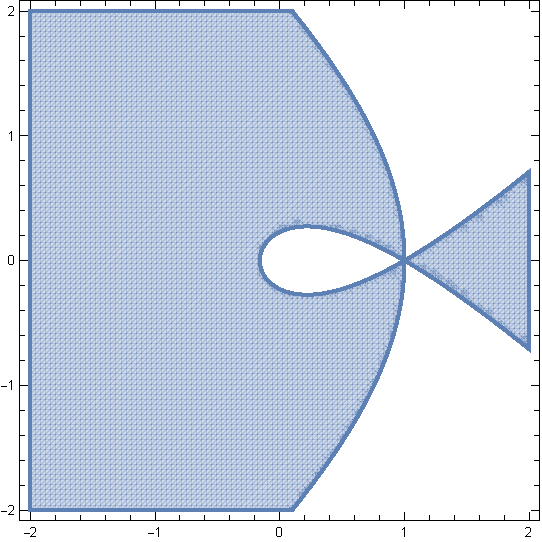
\includegraphics[height=.3\textwidth]{pictures/ReS_edge.pdf}
    \caption{The plot of the region $\operatorname{Re}S(z)-\operatorname{Re}S(1)>0$
			at the edge, in the neighborhood of the double critical point $w_c=1$.
			The new $w$ contour should pass through the shaded region,
		and the new $z$ must stay in the non-shaded region.}
    \label{fig:ReS_edge}
\end{figure}
Note however that the old $z$ contour must encircle $z=a$ and $z=0$,
and $z=a$ is a pole of the integrand. The $w$ contour must always be to the right of
the $z$ contour.

We see that there are three regimes:
\begin{itemize}
	\item If $a<1$, we can deform the $z$ contour to encircle $z=0$ and $z=a$,
		and the $w$ contour to pass through $w=1$. This will lead to the Airy kernel,
		and the derivation is the same as in
		\href{https://lpetrov.cc/rmt25/rmt25-notes/rmt2025-l07.pdf}{Lecture 7}.
		We obtain
		\begin{equation*}
			z=1+\frac{Z}{n^{1/3}},\qquad w=1+\frac{W}{n^{1/3}},\qquad
		\end{equation*}<++>
	\item If $a=1$, the behavior is going to be critical --- we still will
		be able to get the same scaling, but the limiting kernel will be different.
	\item Finally,
\end{itemize}



\begin{remark}
For $\beta=2$ and $a=0$, we typically expand about $z\approx 1$, $w\approx 1$ to capture the top edge at $2\sqrt{t\,n}$.  Indeed, setting $z=1+u,n\to\infty$ leads to the cubic expansions in $u$.
Once $a\neq0$, we get an extra shift in $z$, $w$ that might solve
\[
\partial_z\,\Phi_{t,a}=0,
\quad
\partial_w\,\Phi_{t,a}=0.
\]
We find solutions near $z=1$, $w=1$ if $|a|<2$, but new solutions appear if $|a|>2$.
\end{remark}

\vspace{5pt}

\noindent\textbf{Scaling near the top.}
We know from the unperturbed case $(a=0)$ that $x,y$ near $2\sqrt{t\,n}$ is relevant.  Let us adopt the usual \emph{edge scaling}:
\begin{equation}
\label{eq:xy-edge-scaling}
x \;=\; 2\sqrt{t\,n} \;+\;\frac{\xi}{n^{1/6}},
\qquad
y \;=\; 2\sqrt{t\,n} \;+\;\frac{\eta}{n^{1/6}}.
\end{equation}
Then one can attempt expansions $z=1+u\,n^{-1/3}$, $w=1+v\,n^{-1/3}$ (plus additional shifts if $a\neq0$).  Indeed, if $|a|<2$, the main location for $z_{\mathrm{cr}},w_{\mathrm{cr}}$ remains close to $1$.  Conversely, if $|a|>2$, we get a separate solution.

Let us isolate the product factor first.  Suppose we rewrite
\[
(w-a)\,w^{n-1}
\;=\;
(w-a)\,\exp\bigl((n-1)\ln w\bigr),
\qquad
(z-a)\,z^{n-1}
\;=\;
(z-a)\,\exp\bigl((n-1)\ln z\bigr).
\]
Then
\[
\ln\bigl[(w-a)\,w^{n-1}\bigr] \;=\; (n-1)\ln w \;+\;\ln(w-a).
\]
Hence these combined terms become
\[
(n-1)\,[\ln w-\ln z]
\;+\;
\ln(w-a) \;-\;\ln(z-a).
\]
Because $|a|<2$ or $|a|>2$ drastically changes the location(s) $z-a=0$ or $w-a=0$, the steepest descent approach tries to see where the real part of $\Phi_{t,a}(w,z)$ is stationary.

\subsection{Controlling the integral: subcritical and supercritical analyses}

\subsubsection{Residue crossing and main contributions}

As usual in the $\beta=2$ story, we must deform the $z$-contour outward so that it crosses the $w$-contour.  This can pick up a residue from the simple pole at $w=z$.  In the pure GUE case $(a=0)$, that residue is known to yield the sine or Airy kernel asymptotics after expansions.  Now, with the rank-1 spike, we get an additional factor from $(w-a)/(z-a)$.  The upshot is that \emph{if} the $z$ contour crosses $w$ in a certain region that does not include $w=a$, one obtains a residue that will lead to the same sine/Airy factor.

However, we must also check whether the $z$-contour encloses $z=a$ \emph{and} the $w$-contour encloses $w=a$.  The spike can produce an outlier contribution if $|a|$ is large enough for the new saddle point to dominate.

\subsubsection{Case 1: \texorpdfstring{$|a|<2$}{|a| < 2} (subcritical)}

For $\lvert a\rvert<2$, one can show that the exponent $\Phi_{t,a}(w,z)$ remains effectively minimized near $z,w\approx 1$, and the presence of $(w-a)$ vs.\ $(z-a)$ does not shift that minimizer significantly.  In more precise terms, one writes expansions:
\[
z \;=\; 1 + \frac{u}{n^{1/3}},
\qquad
w \;=\; 1 + \frac{v}{n^{1/3}},
\]
with $x,y$ as in \eqref{eq:xy-edge-scaling}, and obtains a leading cubic term in $u,v$.  The “$a$” correction modifies subleading expansions but does \emph{not} cause a different order in $n$.  Repeating the same steps as in the standard GUE edge analysis (cf.\ \S\ref{sub:double-critical-points}), one sees that the limit of $\frac{1}{n^{1/6}}\,K_t\bigl(x,y\bigr)$ is the Airy kernel
\[
K_{\mathrm{Ai}}(\xi,\eta)
\;=\;
\int_0^\infty \cdots
\]
(as in the usual expression, see \Cref{def:Airy_kernel} for one common form).

Consequently, in the subcritical regime $|a|<2$, the top eigenvalue
\[
x_{\max}(t)= x_1(t)
\]
stays merged in the main bulk near $2\sqrt{t\,n}$ and has \emph{Tracy--Widom} fluctuations on the $n^{-1/6}$ scale.  The factor $a$ only shifts lower-order terms in that expansion.

\subsubsection{Case 2: \texorpdfstring{$|a|>2$}{|a| > 2} (supercritical)}

When $|a|>2$, the spike is large.  One expects an \emph{outlier} eigenvalue near $x\approx a\,\sqrt{t\,}$ (rather than near $2\sqrt{t\,n}$).  Indeed, analyzing $\Phi_{t,a}$ in that scenario, one finds a separate solution to $\partial\Phi/\partial w=0$ near $w\approx a\neq 1$ (and similarly for $z$).  The portion of the $z$-contour around $z= a$ then yields a new local expansion.

Concretely, if $a>2$ (the case $a<-2$ is similar), the factor $(w-a)$ can be near zero, so that the exponent can develop a more favorable real part at $w\approx a$.  Meanwhile, the factor $w^{n-1}$ is enormous if $|w|>1$, but $a>2$ means $|a|>1$.  As a result, the outlier solution with $w\approx a$ can produce a stable stationary phase.  Indeed, one obtains a local \emph{quadratic} expansion around $w=a$ and $z=a$, thus leading to a \emph{Gaussian} fluctuation scale of the resulting outlier eigenvalue, typically $\sigma\,n^{-1/2}$ for some $\sigma>0$.

Hence, in the supercritical regime $|a|>2$, the top eigenvalue $x_{\max}(t)$ \emph{detaches} from $2\sqrt{t\,n}$.  Its leading order becomes $a\sqrt{t\,}$ plus smaller corrections, and the local fluctuations are usually governed by a (shifted) Gaussian (or in some references, an incomplete gamma distribution, depending on subtle normalizations).  The remaining $n-1$ eigenvalues fill out the usual semicircle from $-2\sqrt{t\,n}$ to $2\sqrt{t\,n}$, with an Airy edge near $2\sqrt{t\,n}$.

\subsubsection{Case 3: \texorpdfstring{$|a|=2$}{|a|=2} (critical)}

At the boundary $|a|=2$, the system is at a ``double root'' transition.  One finds that $z=1$ (the standard GUE edge) merges with $z=a$ in a certain sense, leading to a triple or quartic expansion if $a=2$, for instance.  Careful expansions show that the outlier is \emph{just} beginning to separate from the main bulk.  The correlation kernel in this regime is a special transition “higher-order” Airy-like kernel, often described as a \emph{crossover kernel} in the BBP (Baik--Ben~Arous--P\'ech\'e) transition \cite{BBP2005phase}.  The top eigenvalue distribution is neither purely Tracy--Widom nor purely Gaussian but an interpolating limit distribution.

\subsection{Summary of the BBP transition from \texorpdfstring{$K_t(x,y)$}{Kt(x,y)}}

Putting the above cases together, we see that analyzing the DBM correlation kernel
\eqref{eq:K_t_a_expanded} under the spiked initial condition $(a_1=a)\neq0$, $(a_2=\dots=a_n=0)$
reveals:

\begin{itemize}
\item \textbf{If $|a|<2$:}
  The spike is \emph{subcritical}.  The top eigenvalue remains at the GUE edge $\approx 2\sqrt{t\,n}$, with Tracy--Widom fluctuations on scale $n^{-1/6}$.

\item \textbf{If $|a|>2$:}
  The spike is \emph{supercritical}.  An outlier eigenvalue emerges near $a\sqrt{t\,}$, detaching from the main bulk.  The fluctuation scale around that outlier is typically $n^{-1/2}$ and converges (after centering and scaling) to a simpler, often Gaussian-type limit.  The remainder of the spectrum still exhibits the semicircle on $[-2\sqrt{t\,n},2\sqrt{t\,n}]$.

\item \textbf{If $|a|=2$:}
  \emph{Critical regime}.  The top eigenvalue experiences a BBP crossover distribution, with a kernel that can be viewed as a limit of the general \eqref{eq:K_t_a_expanded} by carefully choosing the saddle point expansions.
\end{itemize}

This completes the steepest descent derivation of the rank-1 BBP phase transition from the Dyson Brownian Motion correlation kernel in \Cref{thm:dbm-det-kernel}.  Detailed error estimates and rigorous Fredholm determinant limits (turning kernel statements into actual distributional statements about $x_{\max}(t)$) can be found in \cite{BBP2005phase}, \cite{BloemendalVirag}, and other references cited therein.

\begin{remark}
For $r$-rank spikes (i.e.\ $a_1,\dots,a_r\neq0$), one can repeat the same argument: the factor
$\prod_{i=1}^n (w-a_i)/(z-a_i)$
in \eqref{eq:K_t_a_expanded} splits into a product $(w-a_1)\cdots(w-a_r)\,w^{n-r}$ vs.\ $(z-a_1)\cdots(z-a_r)\,z^{n-r}$.
Each $|a_i|>2$ can produce a distinct outlier, while any $|a_i|<2$ merges with the main bulk.
\end{remark}


















\appendix
\setcounter{section}{10}

\section{Problems (due 2025-04-29)}


\subsection{Biorthogonal ensembles}
\label{prob:biorthogonal}

Derive \Cref{thm:dbm-det-kernel} from
\Cref{lem:density_representation}
using the orthogonalization process similar
to~\href{https://lpetrov.cc/rmt25/rmt25-notes/rmt2025-l05.pdf}{Lecture 5},
and then taking the limit as $s\to\infty$.

\subsection{Scaling of the kernel}
\label{prob:scaling}

Let $a_i=0$ in \Cref{thm:dbm-det-kernel}.
Find $\alpha$ such that
$t^\alpha K_t(x/\sqrt{t},y/\sqrt{t})$ is independent of $t$.
Can you explain this value of $\alpha$?





\bibliographystyle{alpha}
\bibliography{bib}


\medskip

\textsc{L. Petrov, University of Virginia, Department of Mathematics, 141 Cabell Drive, Kerchof Hall, P.O. Box 400137, Charlottesville, VA 22904, USA}

E-mail: \texttt{lenia.petrov@gmail.com}


\end{document}
